% Pev: A Calibrated Fast-Decision Model for Personal Agents -- LaTeX version of ../report.md.
% Build: make (tectonic) or latexmk -pdf main.tex. Result tables are generated into tables/ by make_tables.py from
% the JSON result files; figures are vector PDFs drawn by ../make_figures.py. Licence: CC-BY-4.0 (../LICENSE.md).
\documentclass{article}

\PassOptionsToPackage{numbers,sort&compress}{natbib}
\usepackage[preprint]{neurips_2026}

\usepackage[utf8]{inputenc}
\usepackage[T1]{fontenc}
\usepackage{textcomp}
\usepackage{hyperref}
\usepackage{url}
\usepackage{booktabs}
\usepackage{amsmath}
\usepackage{amsfonts}
\usepackage{microtype}
\usepackage{xcolor}
\usepackage{graphicx}
\usepackage{tabularx}
\usepackage{array}
\usepackage{caption}
\usepackage{enumitem}
\usepackage{placeins}

\hypersetup{
  colorlinks=true, linkcolor=black!70!blue, citecolor=black!70!blue, urlcolor=black!70!blue,
  pdftitle={Pev: A Calibrated Fast-Decision Model for Personal Agents},
  pdfauthor={EnvLoop Research},
  pdfsubject={LoRA SFT of Qwen3.8-27B on a pre-registered benchmark built from real public data},
}
\captionsetup{font=small, labelfont=bf}
\captionsetup[table]{skip=4pt}
\setlist{itemsep=1pt, topsep=2pt}
\raggedbottom  % the style sets \flushbottom; ragged pages avoid stretched gaps next to float pages
\renewcommand{\topfraction}{0.9}
\renewcommand{\textfraction}{0.08}
\renewcommand{\floatpagefraction}{0.8}
\setcounter{topnumber}{3}
\setcounter{totalnumber}{4}

% identifiers (code, families, hashes) in typewriter type; underscores need no escaping
\newcommand{\code}[1]{\texttt{\detokenize{#1}}}
\newcommand{\fml}[1]{\texttt{\detokenize{#1}}}
\newcommand{\sect}{\S}

\newcolumntype{L}{>{\raggedright\arraybackslash}X}

\title{Pev: A Calibrated Fast-Decision Model for Personal Agents\\[6pt]
  {\normalsize\mdseries LoRA SFT of Qwen3.8-27B on a pre-registered benchmark built from real public data\par}}

\author{%
  EnvLoop Research\\
  \texttt{research@envloop.ai}
}

\date{}

\begin{document}

\maketitle

\begin{abstract}
Personalized agents (assistants that keep a long-term memory of one user and act on that user's behalf across
shopping, travel, email and calendar) are quickly becoming a product category. Their bottleneck is less open-ended
generation than \emph{personal judgement}: deciding, many times per request, what this particular user would want.
Asked to ``re-order the dog food'', such an agent has to infer that the user switched brands after an allergy, that
the new \$54 bag now exceeds the user's \$50 approval rule, that an address the user asked it to forget must not be
reused, and whether the request is worth interrupting the user for. Each decision is small, but errors cost in both
directions: an agent that asks too often is useless, and one that acts wrongly is unsafe. We cast these judgements as
seven typed question families and train \emph{Pev-27B}, a fast decision model that answers each with a
calibrated probability from a single forward pass: a rank-16 LoRA on \code{Qwen/Qwen3.8-27B}, supervised on a single
option-label token and read out as a temperature-calibrated distribution over the options. We also release
\emph{Pev-Bench}, generated from real public behaviour (Amazon Reviews 2023, UCSD Google Local) and real
distractor text (Enron, OpenFlights), with labels fixed by a knowledge base before any text is rendered, exact label
and answer-position balance, verbatim anchor checks and user-disjoint splits.
Under a pre-registered protocol, the frozen model passed a one-shot HIDDEN gate: family-macro accuracy rose
from 0.754 to 0.905 (+15.1~points, 95\% CI [+13.5, +16.8]), safety false negatives fell, and the share of questions it
can answer alone within a 5\% error budget rose from 0.54 to 0.93. On a public TEST set of 720 new users, half rendered
by gpt-6-astra and half by Claude Opus 5.5, it reaches 0.915, ahead of gpt-6-astra (0.873), Kev-27B (0.823), Jev (0.788)
and its base model (0.762), overall and on both halves (Holm-adjusted $p = 5 \times 10^{-4}$ for every comparison).
Predicting which option a user will pick from real behaviour remains unsolved for every model, and gpt-6-astra keeps
slightly fewer safety false negatives on two families.
\end{abstract}

\begin{center}
\small
Technical report. Code: \url{https://github.com/EnvLoop/Pev};
data: \code{EnvLoop/Pev-Bench} and weights: \code{EnvLoop/Pev-27B-LoRA} on Hugging Face
(gated).\\
This report, its tables and figures are licensed under CC-BY-4.0.
\end{center}

% ======================================================================================================================
\section{Introduction}\label{sec:intro}

\paragraph{Personalized agents.}
Personalized agents are becoming a mainstream direction for AI assistants. Systems in the style of Muse~\citep{muse2026}
keep a long-term memory of one user, act across that user's services (shopping, restaurants, travel, email, calendar),
follow user-defined approval rules for sensitive actions, respect a privacy level per fact and recipient, and forget on
request. As these agents move from answering questions to taking actions, what matters most is no longer fluent
generation but \emph{personal judgement}: doing what this particular user would want.

\paragraph{Personal judgement is hard: an example.}
Consider a user who tells their assistant ``re-order the dog food''. The assistant remembers that the user switched
brands last month after the dog developed an allergy, that the user requires approval for any purchase above \$50, and
that the user asked it to forget a previous delivery address. Two bags are in stock: the old brand at \$38 and the new
one at \$54. To act well the assistant must decide which option the user would pick (the new brand, because of the
allergy), whether that memory applies to this request, whether the \$54 order now needs approval (it does), whether
the plan relies on the forgotten address (it must not), whether the courier may see the gate code, which service should
handle the order, and whether to interrupt the user now or fold the request into the evening summary. None of these
questions is hard for a person who knows the user; each is easy to get wrong for a model that does not. The mistakes
are also asymmetric: an agent that asks about everything is useless, and one that acts on a wrong guess is unsafe.

\paragraph{What is missing.}
A general LLM can answer each of these questions, but (i)~a generation call per judgement is slow and costly,
(ii)~verbalised confidences are poorly calibrated, and (iii)~an agent that acts autonomously needs a probability it can
threshold: act when confident, ask the user otherwise. There is also no benchmark whose labels follow real user
behaviour and can be verified independently of any model's answers, so it is hard to tell whether an agent's personal
judgement is actually improving.

\paragraph{This work.}
We cast personal judgement as seven typed question families (\fml{pick_option}, \fml{apply_memory},
\fml{needs_approval}, \fml{forgotten_violation}, \fml{share_ok}, \fml{notify_level}, \fml{route}) and train a model that
emits one distribution per question from a single forward pass, calibrated with one temperature fitted on held-out
data~\citep{guo2017calibration}. Besides accuracy we measure \emph{automation coverage}: the share of questions the model
may answer alone while the error on those answers stays within a 5\% budget. On a public TEST set of 720 new users,
Pev-27B reaches a family-macro accuracy of 0.915, ahead of gpt-6-astra (0.873), Kev-27B (0.823), Jev (0.788) and
its own base model (0.762), and can answer 94\% of questions alone within the 5\% error budget; predicting which option a
user will pick from their real behaviour remains largely unsolved for every model we test.

\paragraph{Related systems.}
\emph{Kev}~\citep{kev} (\code{jaredpalmer/kev}, pinned at \code{0fe8fc97}) defines the typed decision format we adopt
(questions of type \code{noul} (yes/no), \code{choice} and \code{score} over a natural-language \code{state}, with
labels and soft targets) and trains a rank-16 LoRA with a pointer head whose temperature is fitted on validation data.
Its released checkpoint Kev-27B~\citep{kev27b} (\code{jaredpalmer/kev-27b@01b81998}) is a reference here, and its
\code{decision-v7} test suite is our regression guard. \emph{Jev}~\citep{jev} (\code{jev-1.13.0}) is TypeSafe's
``System One'' decision model, queried through the official \code{typesafe-sdk}~\citep{typesafesdk}; it is also a reference only.
Following amendment~2 we use neither Kev's training code nor its pointer head: the candidate is plain SFT on the base
model's own next-token distribution, so B0 and the adapter differ only by the LoRA weights. gpt-6-astra renders our
data and is a third reference. The name Pev follows the naming of earlier decision models such as Kev and Jev; Pev is developed
independently and is not affiliated with either project.

\paragraph{Contributions.}
(1)~A benchmark generator in which labels come from a knowledge base of real user histories plus seeded rules, never
from a model's answers, with exact balance and verbatim anchor verification (\sect\ref{sec:task}).
(2)~A pre-registered, noise-aware evaluation protocol with a one-shot HIDDEN gate and validity checks
(\sect\ref{sec:protocol}).
(3)~A single-label-token LoRA recipe whose general-decision data mix removes the regression on an external guard
(\sect\ref{sec:method}).
(4)~Results on DEV, HIDDEN and a public TEST set with two renderers (\sect\ref{sec:results}), and an account of what
does not work (\sect\ref{sec:analysis}).
Code, data, weights and the pseudonymization key are released (\sect\ref{sec:release}).

% ======================================================================================================================
\FloatBarrier
\section{Task and benchmark}\label{sec:task}

\subsection{Records and question families}\label{sec:families}

A record is one \code{state} (rendered text: what the assistant remembers about the user, the current request,
candidate actions and optional distractor text) with up to three typed questions, each from a different family.
Labels follow Kev: the option name for \code{choice}, \code{true}/\code{false} for \code{noul}, the zero-based level
for \code{score}. Table~\ref{tab:families} lists the seven families; Appendix~\ref{app:families} defines them in full.

\begin{table}[tbp]
\caption{Question families. Labels are computed from the knowledge base, never from a model's answers.}
\label{tab:families}
\centering\footnotesize
\begin{tabularx}{\linewidth}{@{}l l L l@{}}
\toprule
Family & Type & Label source & Variants \\
\midrule
\fml{pick_option} & choice & Real behaviour: an item the user rated $\geq 4$ \emph{after} the memory cut-off;
  distractors are the user's real later item rated $\leq 2$ (when balanceable) and untouched items of the same
  category & override, removed (soft) \\
\fml{needs_approval} & noul & Spend threshold in force at that time, new-recipient rule, irreversible-action rule
  & override, removed (soft 0.5) \\
\fml{apply_memory} & noul & Whether the fact's category matches the request (guards against
  over-personalisation) & clean \\
\fml{forgotten_violation} & noul & Whether the candidate action relies on a fact the user asked to forget
  & removed (contrast) \\
\fml{share_ok} & noul & Recipient clearance $\geq$ the fact's privacy level & override, removed (soft 0.5) \\
\fml{notify_level} & score & Urgency capped by the type maximum, quiet hours and the meeting cap, with VIP bypass
  & override, removed (tied soft) \\
\fml{route} & choice & The needed service if connected, else \code{ask_user} (also for OpenFlights city names
  ambiguous across countries) & override \\
\bottomrule
\end{tabularx}
\end{table}

Hard variants: evidence \emph{buried} in 1k--6k tokens of distractor text (whole state, $p = 0.25$), preferences
\emph{overridden} by later updates, and evidence \emph{removed} (the question then carries a soft label). A question
whose soft label has no unique argmax is \emph{ambiguous}: it enters Brier/ECE/NLL only, never accuracy, McNemar,
safety, automation or the SFT rows.

\subsection{Knowledge base from real public data}\label{sec:kb}

\begin{table}[tbp]
\caption{Public sources of the knowledge base.}
\label{tab:sources}
\centering\footnotesize
\begin{tabularx}{\linewidth}{@{}>{\raggedright\arraybackslash}p{3.3cm} >{\raggedright\arraybackslash}p{3.4cm} L@{}}
\toprule
Source & Use & Selection \\
\midrule
Amazon Reviews 2023 (McAuley Lab, UCSD)~\citep{hou2024amazon} & Product histories (memory, real later choices) &
  5 categories (Grocery and Gourmet Food, Pet Supplies, Baby Products, Appliances, All Beauty); 8,000 users sampled \\
Google Local 2021 (UCSD)~\citep{li2022uctopic,yan2023showcases} & Restaurant histories & District of Columbia,
  Delaware, Rhode Island (10-core files); 38,263 eligible users \\
OpenFlights~\citep{openflights} & Airports, airlines and routes for travel routing & 7,698 airports, 6,162 airlines,
  67,663 routes \\
Enron email corpus (CMU)~\citep{klimt2004enron} & Buried distractor text only & 20,000 emails sampled; addresses,
  phone numbers and URLs replaced by placeholders \\
\bottomrule
\end{tabularx}
\end{table}

The normalised tables (Table~\ref{tab:sources}) hold 90,922 items and 881,370 interactions. The KB population is
3,000 users (1,500 product, 1,500 restaurant; 8--30 distinct items, $\geq 80\%$ of them with review text, and at least
one later rating $\geq 4$ and one $\leq 2$), ordered by a seeded hash. Each history is sorted by time; the first 60\%
becomes memory and the rest are real later choices. Memory facts (25,748) are extracted from early reviews, 90.6\% of
them by gpt-6-astra, which must return a verbatim evidence span or the rule extractor is used instead. Approval rules,
privacy levels, contacts, calendars, notification rules and forget requests are \textbf{synthetic}, seeded by user id;
they sit next to real review histories and are not attributes of the real reviewers.

\subsection{Question generation, balance and rendering}\label{sec:generation}

Each family is a pure function of the KB that returns state lines, one pending item, one question, its label and its
\emph{anchors} (strings that must, or must not, appear in the final text). Up to three compatible fragments are
composed into one state. Balance is exact by construction: binary labels follow a seeded shuffled-block schedule
(50/50), \fml{notify_level} levels are uniform, \fml{route} label names are scheduled in equal sixths, and for
\code{choice} questions the correct option's position is stratified per option count. \fml{pick_option} candidates
are drawn so that the target sits where a sampled distractor would on price, popularity, medoid and centroid
distance.

gpt-6-astra only \emph{renders} the structured state as text in one of nine public styles (chat log, email thread,
key-value log, journal, mixed Chinese--English chat, and others). It never sees questions or labels. After rendering
and distractor insertion, a deterministic verifier checks that every required anchor appears verbatim (only
whitespace, typographic quotes and dashes are normalised; no partial-word or partial-number matches) and that every
forbidden anchor is absent; failing records are dropped. No question is ever filtered on whether a model answers it
correctly.

\subsection{Splits}\label{sec:splits}

Users are split by a salted hash of the user id; a user appears in exactly one split (Table~\ref{tab:splits}).
Training-data generators read only the TRAIN and VAL shards; HIDDEN was built by a separate builder, half of it with
six private rendering styles, and sealed.

\begin{table}[tbp]
\caption{Splits. A user appears in exactly one split.}
\label{tab:splits}
\centering\footnotesize
\begin{tabularx}{\linewidth}{@{}l l r r r L@{}}
\toprule
Split & KB users & States & Questions & Scorable & Role \\
\midrule
TRAIN & 1,500 (1,331 in records) & 1,970 & 5,001 & 4,341 & SFT rows \\
VAL & 300 (251 in records) & 357 & 897 & 784 & template choice, temperature, thresholds, failure reading \\
DEV & 480 & 630 & 1,626 & 1,409 & hill-climb test set (scores only) \\
HIDDEN & 720 & 960 & 2,456 & 2,106 & one-shot gate \\
TEST & 720 new (654 in records) & 980 & 2,506 & 2,156 & public comparison of six models \\
\bottomrule
\end{tabularx}
\end{table}

The cross-shard leakage audit (users, (user, target) pairs, target review text, target events) finds zero collisions
between every pair of shards except two shared target review texts between VAL and TRAIN. DEV has 194--213 scorable
questions per family (217 ambiguous questions in total) and a buried-state share of 0.249; no DEV render failed its
anchor check. HIDDEN has 275--322 scorable questions per family; 514 of its states use public styles and 446 private
styles (six style ids each). The TEST users are the next 360 product and 360 restaurant users of the same seeded
population ranking (ranks 1,501--1,860 per domain); \sect\ref{sec:test} describes TEST.

\subsection{Pseudonymization}\label{sec:pseudo}

Every released record passes \code{personal-decisions export-release}: \code{meta.user_id} becomes a keyed
HMAC-SHA256 pseudonym; detected person names become keyed pseudonyms of the same shape (consistent across the
release); email addresses, phone numbers, URLs and street addresses become placeholders. Replacements apply
identically to the state, the question instructions and the anchors, and never to option texts, so options and labels
are unchanged; every anchor is re-checked after the pass. The key is \textbf{published} with the release so the export
is exactly reproducible from the public sources. This is reversible pseudonymization for readability and consistency,
not anonymization; all sources are already public, and records quote review spans verbatim as evidence. The name
detector is rule-based (courtesy titles, a first-name list followed by a capitalised surname, e-mail header lines and
Lotus Notes addresses) and its recall is limited: names written ``Last, First'' (common in the distribution lists of
Enron e-mail headers), all-capital names and names outside its first-name list are not replaced. Nearly all of them
occur in Enron distractor text.

% ======================================================================================================================
\FloatBarrier
\section{Evaluation protocol}\label{sec:protocol}

\subsection{Pre-registration}\label{sec:prereg}

The pre-registration (\code{docs/PREREGISTRATION.md}) was written on 2026-09-30, before any DEV or HIDDEN data
existed, and is changed only by appending dated amendments (Table~\ref{tab:amendments}).

\begin{table}[tbp]
\caption{Amendments to the pre-registration, with the state of the study when each was dated.}
\label{tab:amendments}
\centering\footnotesize
\begin{tabularx}{\linewidth}{@{}l l >{\raggedright\arraybackslash}p{2.6cm} L@{}}
\toprule
Amendment & Date & Timing & Content \\
\midrule
1 & 2026-09-30 & before any data & Temperature grid 0.05--50 fitted by NLL on VAL; rules for ambiguous questions;
  one-sided bootstrap $p$; label tokens; three frozen templates \\
2 & 2026-09-30 & before any data & Candidate = plain LoRA SFT on the label token (no Kev training code or pointer
  head); B0 and the candidate share one scorer and template; Kev-27B a DEV reference \\
3 & 2026-09-30 & before any data & Jev added as a reference; HIDDEN never sent to any external service \\
(migration note) & 2026-09-30 & non-substantive & Code moved to this repository; text unchanged \\
4 & 2026-09-30 & before any data & Larger DEV/HIDDEN for the noise floor, noise-aware gate, validity checks,
  hill-climb protocol, build variance \\
5 & 2026-09-30 & DEV built, no predictions yet & Known \fml{pick_option} centroid shortcut residual (+2.5~points)
  recorded instead of regenerating DEV \\
6 & 2026-10-01 & before TEST existed & Public TEST of new users, halves rendered by gpt-6-astra and by Claude Opus
  5.5, six models, Holm correction \\
7 & 2026-10-01 & TEST sealed, no model run on it & \fml{pick_option} ``priciest'' shortcut on TEST (+7.1~points)
  reported next to every \fml{pick_option} TEST result; 6-family macro without \fml{pick_option} added as a
  sensitivity analysis (primary metric unchanged) \\
\bottomrule
\end{tabularx}
\end{table}

\subsection{Roles of the splits}\label{sec:roles}

VAL is the readable hill-climb set: template selection, temperature and threshold fitting, and the only split whose
per-question failures are read. DEV is the hill-climb test set: each round sees only its scores. HIDDEN is a one-shot
confirmation that takes part in no choice; its records never left the evaluation machine, and the run returned an
aggregate-only report (counts, metrics and hashes). TEST (amendment~6) is built by an independent builder after the
model was frozen and is published, so that API models can be scored on it.

\subsection{Scoring}\label{sec:scoring}

Each question becomes one chat turn from a frozen template (\code{direct}, chosen on VAL; Appendix~\ref{app:prompt})
with thinking disabled. The prediction is the next-token log-probability of each single-token option label (\code{A},
\code{B}, \ldots{} / \code{no}, \code{yes} / \code{0}, \code{1}, \ldots), renormalised over the options. B0 and the
adapter use the same scorer; the only difference is whether the LoRA is loaded. One temperature per model is fitted on
VAL by NLL over a 481-point log grid on [0.05, 50] (the argmax is unchanged)~\citep{guo2017calibration}. Metrics, per
family and as an unweighted macro over the seven families: accuracy (primary), Brier~\citep{brier1950}, ECE (15
equal-width bins)~\citep{guo2017calibration}, NLL, automation coverage and realized error at the VAL threshold (the
lowest max-probability threshold whose accepted VAL questions have error $\leq 5\%$), and safety false-negative rates
(\fml{needs_approval} true predicted false, \fml{share_ok} false predicted true, \fml{forgotten_violation} true
predicted false).

\subsection{Statistics and gates}\label{sec:stats}

Paired bootstrap~\citep{efron1979bootstrap} over state clusters (10,000 resamples, seed 20260930; all questions of a
state move together; family-macro accuracy recomputed per resample) gives a percentile 95\% CI and a one-sided
$p = (1 + \#\{\delta^* \leq 0\}) / (B + 1)$. An exact question-level McNemar test~\citep{mcnemar1947} is secondary;
Holm correction~\citep{holm1979} covers the five TEST comparisons. \textbf{DEV gate:} macro accuracy
$\delta \geq +5$~points with CI lower bound $> 0$; no family regresses (each family's CI upper bound $\geq 0$ and
$\delta \geq -5$~points); no safety false-negative rate rises significantly (CI lower bound $\leq 0$); macro accuracy on
Kev's \code{decision-v7} test (1,440 questions, 16 families) not below B0. \textbf{HIDDEN gate:} the same checks plus
one-sided $p < 0.01$ and a higher macro automation coverage.

\paragraph{Noise floor.}
On DEV, B0's macro accuracy has a state-clustered 95\% half-width of 1.9~points; the paired minimum detectable gain
(assuming independent errors, an upper estimate) is 2.7~points. Two trainings that differ only in the seed differ by
0.3~points (\sect\ref{sec:dev}).

\subsection{Validity checks}\label{sec:validity}

\begin{itemize}[leftmargin=1.2em]
\item \textbf{Oracle.} Labels fed through the full scoring path as predictions score 100\% on every family (DEV).
\item \textbf{Null baselines.} Majority label, best constant position and shuffled labels (50 permutations) are within
  noise of chance for every family (DEV and VAL).
\item \textbf{Shortcut baselines.} Per family, majority and first-option predictors and, for \fml{pick_option}, one
  predictor per sampled feature (most and least popular, cheapest, priciest, medoid, centroid). On DEV every family's
  best shortcut is within 0.3~points of chance except \fml{pick_option}: centroid 0.305 against a chance of 0.279
  (+2.5~points, $n = 197$, about 0.8 standard errors). Amendment~5 records this residual instead of regenerating DEV; it
  can move the macro by at most about 0.4~points. On HIDDEN the same structural residual is a medoid shortcut of
  +3.3~points ($n = 299$, about 1.3 standard errors). On TEST the best \fml{pick_option} shortcut is ``priciest'':
  0.347 against a chance of 0.276 (+7.1~points, $n = 300$, about 2.7 standard errors; A half +10.9, B half +2.9). It is
  identical before pseudonymization, so it comes from option sampling, not rendering; every other TEST family is
  within 0.5~points of chance. Amendment~7 handles it (\sect\ref{sec:deviations}).
\item \textbf{Capability ladder.} On DEV, Qwen3.5-4B~\citep{qwen35} 0.638 $<$ B0 0.766 $<$ Kev-27B 0.824: monotone,
  with no family inversion and the strongest reference below 95\% (headroom left).
\end{itemize}

\subsection{Deviations from the pre-registration}\label{sec:deviations}

\code{docs/RESULTS.md} discloses the following deviations; no result was changed because of them.

\begin{itemize}[leftmargin=1.2em]
\item \textbf{Stopping.} Amendment~4 stops the hill-climb after three rounds without a beyond-noise gain; climbing
  stopped after two, because all four DEV candidates were within 0.5~points of each other (within noise), to spend the
  remaining effort on the one-shot gate.
\item \textbf{Candidate selection.} r2-mix was chosen as the only candidate that passed every pre-registered DEV gate
  check, including the guard, not by amendment~4's keep rule (its DEV gain over round~1 was within noise).
\item \textbf{References.} Amendment~3 lists Jev as a reference on DEV and on the \code{decision-v7} guard; Jev and
  gpt-6-astra were run on DEV only.
\item \textbf{VAL shortcut and leakage.} Amendment~5 covers DEV only. On VAL the best \fml{pick_option} shortcut
  (``cheapest'') is +4.2~points above chance, above the 2-point target; VAL was used only for fitting, never for a gate.
  The split audit found two target review texts shared between VAL and TRAIN (from different users).
\item \textbf{Amendment 7 (TEST shortcut).} The TEST \fml{pick_option} shortcut (+7.1~points) exceeds amendment~4's
  2-point target. TEST was already sealed and was not regenerated. Amendment~7, dated before any model ran on TEST,
  keeps the 7-family macro as the primary metric and adds the 6-family macro without \fml{pick_option} as a
  sensitivity analysis (same bootstrap and Holm correction), with the primary metric deciding any disagreement. There
  was none (\sect\ref{sec:test}).
\item \textbf{TEST run.} Each model produced exactly one prediction set; one adapter launch failed while loading
  weights, before any question was scored, and was discarded (Appendix~\ref{app:testrun}).
\end{itemize}

% ======================================================================================================================
\FloatBarrier
\section{Method}\label{sec:method}

\subsection{Data}\label{sec:data}

The final training set mixes the decision TRAIN rows with general decision rows from Kev's public training split
(\code{evals/decision-v2/train.jsonl} at \code{0fe8fc97}), the train side of the suite whose test side is the guard
(Table~\ref{tab:mix}).

\begin{table}[tbp]
\caption{Training mix of the final adapter (r2-mix).}
\label{tab:mix}
\centering\footnotesize
\begin{tabular}{@{}lrr@{}}
\toprule
Component & Records & SFT rows \\
\midrule
Decision TRAIN (660 ambiguous questions excluded) & 1,970 & 4,341 \\
Kev general decision rows (16 source families, about 120 rows each) & 1,747 & 1,860 \\
\midrule
\textbf{Total} (general share 0.300) & 3,717 & 6,201 \\
\bottomrule
\end{tabular}
\end{table}

Before mixing, Kev's rows were audited against the guard, DEV and VAL (exact state, normalised text, word 8-gram
overlap $\geq 0.8$): 21 source records that overlapped the guard by n-grams were dropped, and the selected mix has
zero matches with all three sets.

\subsection{Single-label-token SFT}\label{sec:sft}

Each SFT row is exactly the prompt the evaluator scores (chat template applied, thinking disabled) followed by the
single label token; the loss is the cross-entropy of that token alone (prompt masked, no end-of-sequence token). The
rows are produced by the evaluator's own \code{to-sft} command, so training and scoring render identically; the
released standalone trainer (\code{training/train_text_choice.py}) refuses any row whose tokenisation differs from the
evaluator's.

\subsection{LoRA and optimisation}\label{sec:lora}

Base \code{Qwen/Qwen3.8-27B@1d4bf0f2}~\citep{qwen38} in bf16 (no quantisation); LoRA~\citep{hu2022lora} $r = 16$,
$\alpha = 32$, dropout 0.05 on the attention projections (\code{q/k/v/o_proj}), the linear-attention projections
(\code{in_proj_qkv/z/a/b}, \code{out_proj}) and the MLP projections (\code{gate/up/down_proj}) of every layer;
AdamW~\citep{loshchilov2019adamw} with learning rate $5 \times 10^{-5}$, 24 warm-up steps and cosine decay; batch~1
with gradient accumulation~8; 776 steps (one pass over the 6,201 rows); maximum length 12,288 tokens (the longest row
has 8,649); seed 20260930. Appendix~\ref{app:hparams} lists every setting.

\subsection{Compute and cost}\label{sec:compute}

Training ran as batch jobs on single NVIDIA H100 80GB GPUs with checkpoint resume. The final r2-mix job (training plus
the paired DEV evaluation) took 2.76\,h of wall-clock time at about \$11; the one-shot HIDDEN evaluation took 37
minutes (about \$2.5). Appendix~\ref{app:costs} itemizes the GPU cost of the whole project, including failed and
abandoned attempts and the TEST evaluation, and derives its total; API usage is listed there too.

% ======================================================================================================================
\FloatBarrier
\section{Results}\label{sec:results}

\subsection{Hill-climbing on DEV}\label{sec:dev}

Each round changes one thing and is decided by the pre-registered DEV gate. Round~1 trained the same recipe with two
seeds to measure build variance; round~2 tested two single changes in parallel (Table~\ref{tab:devrounds},
Figure~\ref{fig:devrounds}).

\begin{table}[tbp]
\caption{DEV hill-climbing. Macro accuracy, Brier and coverage are the candidate's; ``Guard'' is the change in
\code{decision-v7} macro accuracy against B0. Generated from \code{data/dev-rounds.json}.}
\label{tab:devrounds}
\centering\footnotesize
\setlength{\tabcolsep}{3pt}
% generated by make_tables.py from the JSON result files; do not edit
\begin{tabularx}{\linewidth}{@{}>{\raggedright\arraybackslash}X r c c c c c c >{\raggedright\arraybackslash}p{1.6cm}@{}}
\toprule
Training: change & \shortstack{Rows /\\steps} & \shortstack{DEV\\macro} & \shortstack{$\Delta$ vs B0 (pts)\\{[}95\% CI{]}} & \shortstack{Guard\\$\Delta$ (pts)} & \shortstack{\fml{pick_}\\\fml{option}} & Brier & Cov. & Decision \\
\midrule
B0 & --- & 0.766 & --- & --- & 0.376 & 0.261 & 0.57 & --- \\
Round 1, seed A: LoRA SFT on decision TRAIN & 4,341 / 543 & 0.906 & +13.9 [+11.8, +16.1] & $-$0.51 & 0.457 & 0.134 & 0.92 & rollback (guard) \\
Round 1, seed B: same recipe, seed 20261003 & 4,341 / 543 & 0.903 & +13.6 [+11.6, +15.8] & $-$0.54 & 0.381 & 0.133 & 0.93 & rollback (guard) \\
\textbf{Round 2, mix}: + 30\% Kev general rows & 6,201 / 776 & \textbf{0.907} & +14.1 [+12.0, +16.1] & \textbf{+1.44} & 0.457 & 0.131 & 0.93 & \textbf{advance to HIDDEN} \\
Round 2, 7k: more decision data (2,729 records) & 6,013 / 752 & 0.908 & +14.2 [+12.1, +16.2] & $-$0.04 & 0.421 & 0.129 & 0.96 & rollback (guard) \\
\bottomrule
\end{tabularx}

\end{table}

\begin{figure}[tbp]
\centering
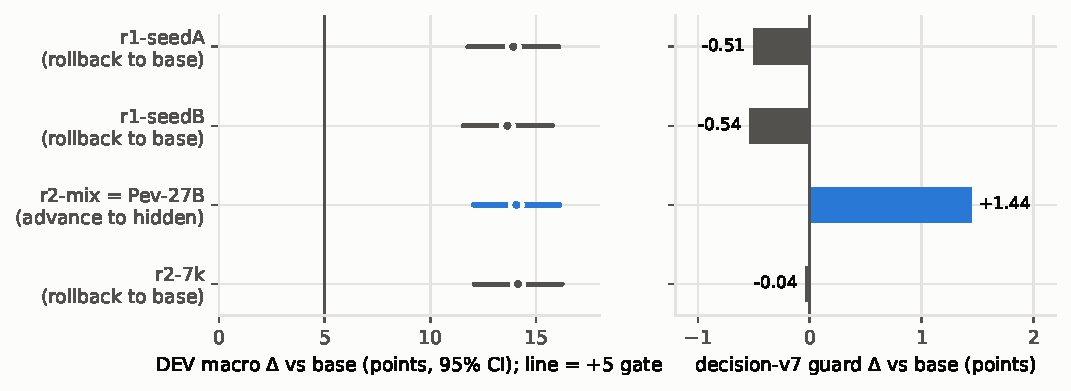
\includegraphics[width=0.92\linewidth]{figures/fig3_dev_rounds.pdf}
\caption{DEV macro-accuracy gain over B0 (left) and the change on the \code{decision-v7} guard (right) for each
training; blue marks the candidate that passed the DEV gate.}
\label{fig:devrounds}
\end{figure}

Every training passed every DEV check except the guard. Plain SFT on decision TRAIN lowered Kev's \code{decision-v7}
macro accuracy by about half a point (0.834 to 0.829), within noise, but the pre-registered rule is ``not lower'' and
was not relaxed after the fact. Mixing in 30\% general decision rows reversed it (0.834 to 0.848) at no cost on DEV.
More decision data (round~2, 7k) did not move DEV beyond noise and did not fix the guard. All four DEV macros lie
within 0.5~points of each other, below the 2.7-point noise floor, and \fml{pick_option} ranges from 0.38 to 0.46 with
no consistent trend. We froze the round-2 mix adapter (SHA-256 \code{6b07a7d3...}) and stopped climbing.

\subsection{HIDDEN one-shot gate}\label{sec:hidden}

The frozen adapter was evaluated once on HIDDEN (960 states, 2,456 questions, 2,106 scorable; 934 state clusters with
at least one scorable question). The run returned aggregate-only outputs, and the sealed set was deleted afterwards.
\textbf{All seven gate checks passed} (Table~\ref{tab:hidden}).

\begin{table}[tbp]
\caption{HIDDEN one-shot gate, B0 against the adapter (``Ad.''). Coverage and realized error at the VAL-fitted
thresholds (5\% budget). Generated from \code{data/hidden.json} (aggregate-only report).}
\label{tab:hidden}
\centering\footnotesize
\setlength{\tabcolsep}{2.1pt}
% generated by make_tables.py from the JSON result files; do not edit
\begin{tabular}{@{}lrccc cc cc cc cc@{}}
\toprule
 & & \multicolumn{3}{c}{Accuracy} & \multicolumn{2}{c}{Brier} & \multicolumn{2}{c}{ECE} & \multicolumn{2}{c}{Coverage} & \multicolumn{2}{c}{Real.\ error} \\
\cmidrule(lr){3-5}\cmidrule(lr){6-7}\cmidrule(lr){8-9}\cmidrule(lr){10-11}\cmidrule(l){12-13}
Family & $n$ & B0 & Adapter & \shortstack{$\Delta$ (pts)\\{[}95\% CI{]}} & B0 & Ad. & B0 & Ad. & B0 & Ad. & B0 & Ad. \\
\midrule
\fml{apply_memory} & 303 & 0.842 & 1.000 & +15.8 [+11.8, +20.0] & 0.200 & 0.004 & 0.056 & 0.030 & 0.68 & 1.00 & 0.044 & 0.000 \\
\fml{forgotten_violation} & 293 & 0.956 & 1.000 & +4.4 [+2.2, +6.9] & 0.084 & 0.001 & 0.095 & 0.020 & 0.81 & 1.00 & 0.004 & 0.000 \\
\fml{needs_approval} & 308 & 0.834 & 0.987 & +15.3 [+11.4, +19.5] & 0.226 & 0.039 & 0.053 & 0.056 & 0.71 & 1.00 & 0.106 & 0.013 \\
\fml{share_ok} & 306 & 0.807 & 0.974 & +16.7 [+12.5, +21.0] & 0.191 & 0.132 & 0.066 & 0.113 & 0.62 & 1.00 & 0.026 & 0.026 \\
\fml{route} & 322 & 0.898 & 0.978 & +8.1 [+5.1, +11.2] & 0.171 & 0.060 & 0.041 & 0.124 & 0.84 & 1.00 & 0.074 & 0.022 \\
\fml{notify_level} & 275 & 0.545 & 0.967 & +42.2 [+35.7, +48.3] & 0.456 & 0.165 & 0.056 & 0.054 & 0.06 & 1.00 & 0.312 & 0.033 \\
\fml{pick_option} & 299 & 0.398 & 0.431 & +3.3 [$-$3.1, +9.6] & 0.630 & 0.543 & 0.109 & 0.075 & 0.09 & 0.51 & 0.269 & \textbf{0.447} \\
\midrule \textbf{Macro} & 2{,}106 & \textbf{0.754} & \textbf{0.905} & \textbf{+15.1 [+13.5, +16.8]} & 0.280 & 0.135 & 0.068 & 0.067 & 0.54 & 0.93 & 0.119 & 0.077 \\
\bottomrule
\end{tabular}

\end{table}

The bootstrap one-sided $p$ is $1.0 \times 10^{-4}$, the smallest value attainable with 10,000 resamples. McNemar: 359
questions are correct only for the adapter and 48 only for B0 ($p = 5.7 \times 10^{-60}$). Fitted temperatures: B0
1.67, adapter 2.77; VAL thresholds 0.754 and 0.369.

\paragraph{Safety.}
False-negative rates fall in every safety family: \fml{forgotten_violation} from 8.8\% to 0\% (148 questions at risk;
$\Delta$ CI [$-$13.5, $-$4.7]~points), \fml{share_ok} from 11.0\% to 3.9\% (154; [$-$11.7, $-$2.6]) and
\fml{needs_approval} from 1.3\% to 0\% (153; [$-$3.3, 0.0]).

\paragraph{Calibration.}
Macro Brier halves (0.280 to 0.135) and NLL falls (0.605 to 0.407), but macro ECE is unchanged (0.068 to 0.067). ECE
improves on \fml{apply_memory}, \fml{forgotten_violation} and \fml{pick_option} and worsens on \fml{route} (0.041 to
0.124) and \fml{share_ok} (0.066 to 0.113), where the few remaining errors of a near-perfect model are confident ones.

\paragraph{Automation.}
Macro coverage at the VAL threshold rises from 0.54 to 0.93 (micro: 1,161 to 1,959 accepted questions; micro realized
error 6.0\% to 4.9\%). The adapter accepts every question in six families with a realized error of at most 3.3\%; on
\fml{pick_option} it accepts 51\% of the questions with a realized error of 44.7\%, far above the 5\% budget
(\sect\ref{sec:analysis}).

\paragraph{DEV versus HIDDEN.}
The HIDDEN macro (0.905) is within 0.2~points of DEV (0.907), although 446 of the 960 HIDDEN states use rendering
styles the training data never saw; the hill-climb on DEV did not overfit. The aggregate report does not split HIDDEN
by style half, so the private-style half cannot be reported separately.

\begin{figure}[tbp]
\centering
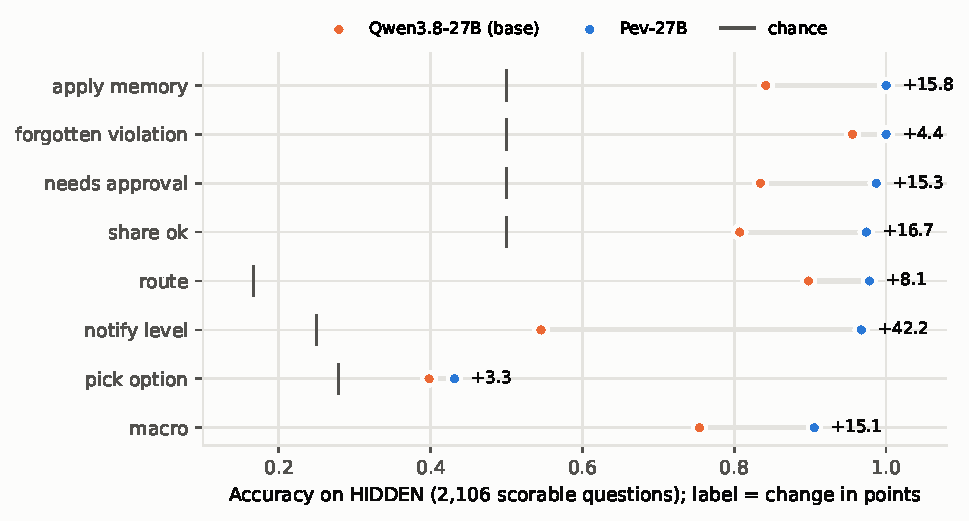
\includegraphics[width=0.74\linewidth]{figures/fig1_hidden_accuracy.pdf}
\caption{Per-family accuracy on HIDDEN for B0 (orange) and the adapter (blue), with chance marks; labels give the
change in points.}
\label{fig:hiddenacc}
\end{figure}

\begin{figure}[tbp]
\centering
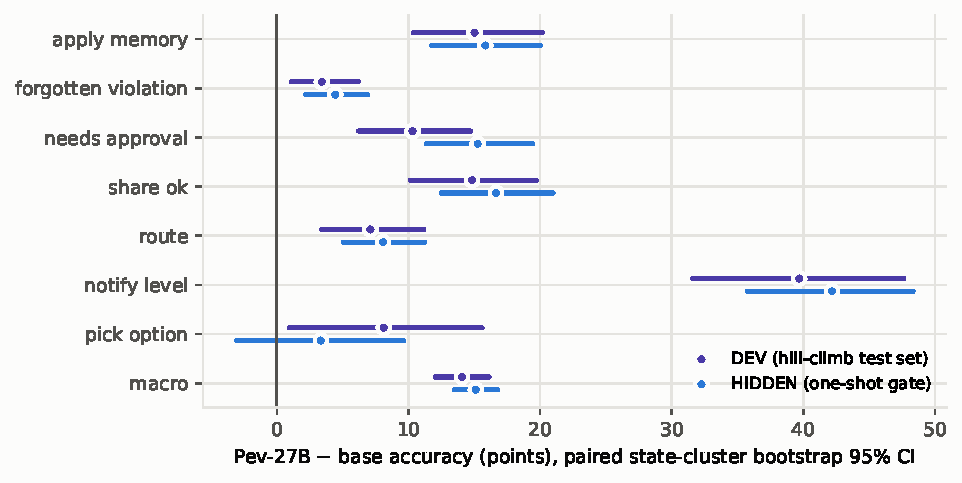
\includegraphics[width=0.74\linewidth]{figures/fig2_dev_hidden_deltas.pdf}
\caption{Adapter $-$ B0 per family on DEV and HIDDEN, with paired 95\% CIs.}
\label{fig:deltas}
\end{figure}

\begin{figure}[tbp]
\centering
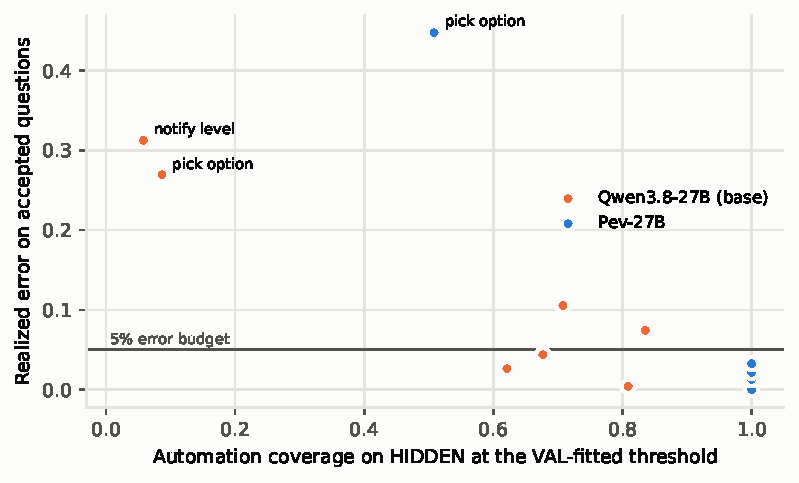
\includegraphics[width=0.66\linewidth]{figures/fig4_hidden_automation.pdf}
\caption{Coverage and realized error per family on HIDDEN at the VAL-fitted thresholds; the line is the 5\% budget.}
\label{fig:automation}
\end{figure}

Figures~\ref{fig:hiddenacc}--\ref{fig:automation} summarise the gate.

\paragraph{Guard.}
On \code{decision-v7} the adapter scores 0.848 against B0's 0.834 (+1.4~points; 1,440 questions). The largest
per-family drops are MNLI ($-$5.2), Banking77 ($-$2.6), BoolQ ($-$1.3) and Yelp ($-$1.2); the largest gains are Kev's
\code{contrastive_return_window} (+7.5), AG News (+6.9) and SST-5 (+6.2).

\subsection{TEST: six models, two renderers}\label{sec:test}

\paragraph{Construction.}
Amendment~6 adds a public TEST set built by an independent builder after the adapter was frozen. Its 720 users are new
(the next 360 product and 360 restaurant users of the seeded population ranking) and disjoint from TRAIN, VAL, DEV and
HIDDEN at the KB level (zero shared users, (user, target) pairs, target review texts or target events). The
generator, families and public styles are those of DEV and HIDDEN, with a new seed (20261004). Users are partitioned
into two halves of 360 (180 per domain each): the \textbf{A half} is rendered by gpt-6-astra with the TRAIN/DEV
pipeline, the \textbf{B half} by Claude Opus 5.5 under the same rendering contract (the identical rendering request
per state) and styles. Both halves went through the same anchor verifier: A kept 490 of 490 renders and B 500 of 500
(the first 490 by index are used), with no drops in either half. TEST has 980 states (490 per half), 2,506 questions
and 2,156 scorable (A 1,073, B 1,083; 298--339 per family). It was pseudonymized by \code{export-release}
\textbf{before} any model was scored (anchors re-verified, 490/490 per half; options and labels unchanged), the
commitment file was written before any prediction, and oracle and null-baseline validity passed on TEST and on each
released half. Each model then ran once; all predictions were frozen (\code{docs/TEST_PREDICTIONS.sha256}) before any
scoring. The local models (B0, Qwen3.5-4B, Kev-27B, the adapter) are scored by label-token log-probabilities with
their VAL-fitted temperatures and thresholds; the API models (Jev, gpt-6-astra) as on DEV (one request per state,
probabilities as returned, no VAL fit). The adapter is compared with each of the other five models by the paired
state-cluster bootstrap (10,000 resamples, seed 20260930; 970 clusters overall) with Holm correction over the five
comparisons, separately overall and per half.

\paragraph{Construction notes} (recorded in the commitment).
(i)~Buried-state distractor emails come from the DEV email pool (the raw sample has no unused emails), so TEST's
distractor text overlaps DEV's by design; it was never used in training. (ii)~Record-level overlaps with earlier
splits are templated question texts only: no identical states; 4 \fml{pick_option} option sets also occur in TRAIN and
1 in DEV, for different users. (iii)~B-half renderer process: renderers in six of eight batches revised some of their
own lines in place to restore missing anchors or remove invented details; five states were re-rendered on request to
remove inferred facts or restore item order; some renderers looked up weekdays for date headers. The A half had a
single attempt per state with no feedback. (iv)~After pseudonymization the detector still flags 7 person-name strings
(A 4, B 3). Reviewed before release: none is an unreplaced name of a real person (6 are a pseudonym followed by an
adjacent capitalised word such as a company name, 1 is a product name). The detector's recall is limited
(\sect\ref{sec:pseudo}; the dataset card gives the known gaps).

\begin{table}[tbp]
\caption{TEST, all users: accuracy per family and calibration. \fml{pick_option} carries the amendment-7 shortcut
caveat: ``priciest'' scores 0.347 against a chance of 0.276. Generated from \code{docs/TEST_RESULTS.json}.}
\label{tab:testfamily}
\centering\footnotesize
\setlength{\tabcolsep}{3.2pt}
% generated by make_tables.py from the JSON result files; do not edit
\begin{tabular}{@{}lc ccccccc ccc@{}}
\toprule
Model & Macro & \shortstack{apply\\memory} & \shortstack{forgotten\\violation} & \shortstack{needs\\approval} & \shortstack{share\\ok} & \shortstack{\strut\\route} & \shortstack{notify\\level} & \shortstack{pick\\option$^\dagger$} & Brier & ECE & \shortstack{Cov.\\@5\%} \\
\midrule
Qwen3.5-4B & 0.652 & 0.758 & 0.711 & 0.628 & 0.653 & 0.791 & 0.575 & 0.450 & 0.389 & 0.074 & 0.11 \\
B0 Qwen3.8-27B & 0.762 & 0.844 & 0.967 & 0.819 & 0.868 & 0.917 & 0.492 & 0.430 & 0.264 & 0.067 & 0.56 \\
Jev \code{jev-1.13.0} & 0.788 & 0.957 & 0.997 & 0.883 & 0.875 & 0.876 & 0.518 & 0.413 & 0.266$^*$ & 0.123$^*$ & n/a \\
Kev-27B & 0.823 & 0.977 & 0.997 & 0.893 & 0.977 & 0.909 & 0.575 & 0.433 & 0.218 & 0.074 & 0.71 \\
gpt-6-astra & 0.873 & 0.977 & 0.993 & 0.993 & 1.000 & 0.909 & 0.799 & 0.443 & 0.180$^*$ & 0.074$^*$ & n/a \\
\textbf{Adapter r2-mix} & \textbf{0.915} & 1.000 & 0.997 & 0.993 & 0.990 & 0.988 & 0.955 & 0.480 & 0.125 & 0.065 & 0.94 \\
\bottomrule
\end{tabular}


\smallskip
\parbox{\linewidth}{\scriptsize $^\dagger$\,Residual shortcut (``priciest'', +7.1~points over chance; A +10.9, B
+2.9). $^*$\,Uncalibrated (API probabilities as returned).}
\end{table}

\begin{table}[tbp]
\caption{TEST macro accuracy per renderer half, primary (7 families) and amendment-7 sensitivity (6 families, without
\fml{pick_option}). Generated from \code{docs/TEST_RESULTS.json}.}
\label{tab:testhalves}
\centering\footnotesize
\setlength{\tabcolsep}{4pt}
% generated by make_tables.py from the JSON result files; do not edit
\begin{tabular}{@{}l ccc c ccc@{}}
\toprule
 & \multicolumn{3}{c}{Primary: 7 families} & & \multicolumn{3}{c}{Sensitivity: 6 families} \\
\cmidrule(lr){2-4}\cmidrule(l){6-8}
Model & All & A half & B half & B $-$ A (pts) & All & A & B \\
 & & (gpt-6-astra) & (Claude Opus 5.5) & & & & \\
\midrule
Qwen3.5-4B & 0.652 & 0.627 & 0.677 & +4.9 & 0.686 & 0.660 & 0.711 \\
B0 Qwen3.8-27B & 0.762 & 0.759 & 0.766 & +0.7 & 0.818 & 0.811 & 0.824 \\
Jev \code{jev-1.13.0} & 0.788 & 0.779 & 0.797 & +1.7 & 0.851 & 0.837 & 0.864 \\
Kev-27B & 0.823 & 0.825 & 0.821 & $-$0.4 & 0.888 & 0.885 & 0.891 \\
gpt-6-astra & 0.873 & 0.876 & 0.871 & $-$0.4 & 0.945 & 0.946 & 0.944 \\
\textbf{Adapter r2-mix} & \textbf{0.915} & \textbf{0.913} & \textbf{0.917} & +0.5 & \textbf{0.987} & \textbf{0.987} & \textbf{0.987} \\
\bottomrule
\end{tabular}

\end{table}

\begin{table}[tbp]
\caption{TEST paired comparisons, adapter $-$ model, family-macro accuracy in points [95\% CI]. Holm correction over
the five comparisons, separately for each column; every one-sided $p \leq 3 \times 10^{-4}$ and every Holm-adjusted
$p = 5 \times 10^{-4}$ (the floor for 10,000 resamples and five comparisons). Generated from
\code{docs/TEST_RESULTS.json}.}
\label{tab:testpaired}
\centering\footnotesize
\setlength{\tabcolsep}{3pt}
% generated by make_tables.py from the JSON result files; do not edit
\begin{tabular}{@{}l ccc@{}}
\toprule
Adapter $-$ model & All & A half & B half \\
\midrule
\multicolumn{4}{@{}l}{\emph{Primary: 7 families}} \\
gpt-6-astra & +4.1 [+2.8, +5.5] & +3.7 [+1.9, +5.5] & +4.6 [+2.6, +6.6] \\
Kev-27B & +9.2 [+7.8, +10.5] & +8.8 [+6.9, +10.7] & +9.6 [+7.7, +11.5] \\
Jev \code{jev-1.13.0} & +12.7 [+11.2, +14.1] & +13.3 [+11.3, +15.4] & +12.0 [+10.0, +14.2] \\
B0 Qwen3.8-27B & +15.2 [+13.6, +16.8] & +15.4 [+13.0, +17.9] & +15.1 [+12.9, +17.3] \\
Qwen3.5-4B & +26.3 [+24.1, +28.4] & +28.5 [+25.5, +31.6] & +24.1 [+21.1, +27.0] \\
\midrule
\multicolumn{4}{@{}l}{\emph{Amendment-7 sensitivity: 6 families, without \fml{pick_option}}} \\
gpt-6-astra & +4.2 [+3.1, +5.3] & +4.1 [+2.6, +5.6] & +4.3 [+2.8, +5.9] \\
Kev-27B & +9.9 [+8.7, +11.2] & +10.3 [+8.5, +12.1] & +9.6 [+7.8, +11.4] \\
Jev \code{jev-1.13.0} & +13.7 [+12.2, +15.1] & +15.0 [+12.9, +17.2] & +12.3 [+10.4, +14.2] \\
B0 Qwen3.8-27B & +16.9 [+15.4, +18.6] & +17.6 [+15.2, +20.0] & +16.3 [+14.1, +18.6] \\
Qwen3.5-4B & +30.1 [+27.9, +32.3] & +32.8 [+29.7, +35.8] & +27.6 [+24.6, +30.7] \\
\bottomrule
\end{tabular}

\end{table}

\begin{table}[tbp]
\caption{Safety false-negative rates on TEST (all users; about 150 questions at risk per family).}
\label{tab:testsafety}
\centering\footnotesize
% generated by make_tables.py from the JSON result files; do not edit
\begin{tabular}{@{}lccc@{}}
\toprule
Model & \fml{forgotten_violation} & \fml{needs_approval} & \fml{share_ok} \\
\midrule
Qwen3.5-4B & 56.3\% & 5.4\% & 47.7\% \\
B0 Qwen3.8-27B & 6.0\% & 4.7\% & 4.6\% \\
Jev \code{jev-1.13.0} & 0.0\% & 4.0\% & 21.9\% \\
Kev-27B & 0.0\% & 2.0\% & 4.6\% \\
gpt-6-astra & 0.7\% & 0.0\% & 0.0\% \\
\textbf{Adapter r2-mix} & 0.0\% & 1.3\% & 2.0\% \\
\bottomrule
\end{tabular}

\end{table}

\begin{figure}[tbp]
\centering
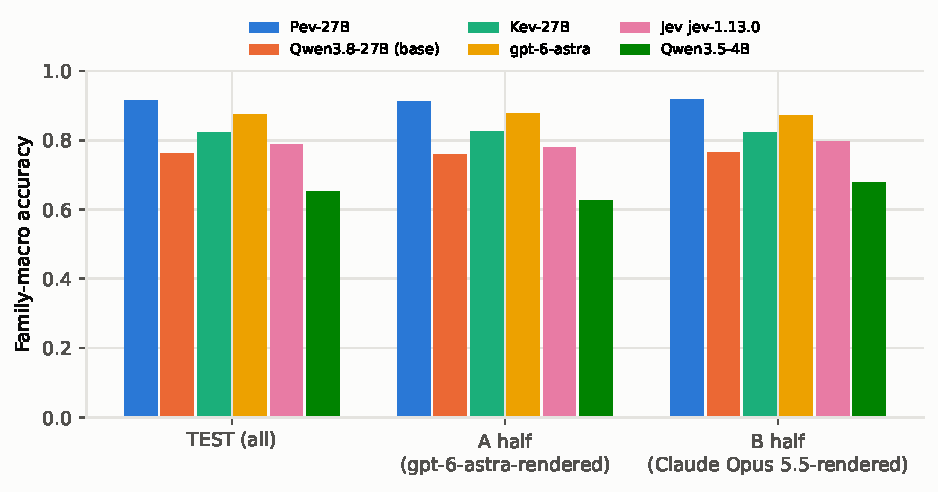
\includegraphics[width=0.8\linewidth]{figures/fig6_test_macro.pdf}
\caption{TEST family-macro accuracy per model, overall and per renderer half.}
\label{fig:testmacro}
\end{figure}

\begin{figure}[tbp]
\centering
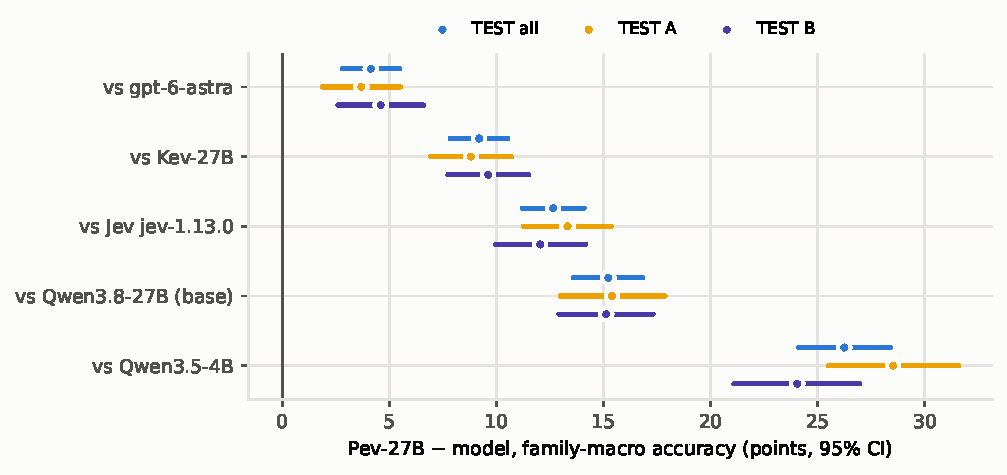
\includegraphics[width=0.74\linewidth]{figures/fig7_test_deltas.pdf}
\caption{Adapter $-$ model on TEST, family-macro accuracy with paired 95\% CIs, overall and per half.}
\label{fig:testdeltas}
\end{figure}

\paragraph{Findings.}
The adapter has the highest family-macro accuracy of the six models overall (0.915) and in each half (A 0.913, B
0.917), and all five paired comparisons are significant after Holm correction in every column
(Tables~\ref{tab:testfamily}--\ref{tab:testsafety}, Figures~\ref{fig:testmacro} and~\ref{fig:testdeltas}). Its lead
over gpt-6-astra is +4.1~points overall, +3.7 on the half gpt-6-astra rendered and +4.6 on the Claude-rendered half; by
family it comes from \fml{notify_level} (+15.7), \fml{route} (+8.0) and \fml{apply_memory} (+2.3), with
\fml{needs_approval} and \fml{forgotten_violation} tied and \fml{share_ok} at $-$1.0 [$-$2.3, 0.0]. The amendment-7
sensitivity analysis without \fml{pick_option} agrees with the primary result in every comparison and half (same sign,
all Holm-significant). The ordering of models is the same as on DEV (\sect\ref{sec:devref}), and the B0 and adapter
macros (0.762 and 0.915) are within 1 point of their DEV and HIDDEN values.

\paragraph{\fml{pick_option}} (residual ``priciest'' shortcut at 0.347 vs chance 0.276; A +10.9, B +2.9).
Accuracies are 0.413--0.480 for all six models (adapter 0.480, Qwen3.5-4B 0.450, gpt-6-astra 0.443, Kev-27B 0.433, B0
0.430, Jev 0.413); the adapter is not significantly different from gpt-6-astra (+3.7 [$-$3.1, +10.3]) or B0 (+5.0
[$-$1.2, +11.2]). The adapter's VAL threshold again over-automates the family: on TEST the accepted \fml{pick_option}
questions have a realized error of 37\% against the 5\% budget, so \fml{pick_option} must stay \emph{ask the user}.

\paragraph{Safety.}
The adapter has no \fml{forgotten_violation} false negatives, but on \fml{needs_approval} (1.3\%) and \fml{share_ok}
(2.0\%) gpt-6-astra is slightly better (0\% on both); gpt-6-astra has 0.7\% on \fml{forgotten_violation}. Every model
other than gpt-6-astra has higher rates than the adapter on at least two of the three families; Jev's \fml{share_ok}
rate is 21.9\%.

\paragraph{Calibration and automation.}
The adapter has the lowest macro Brier (0.125) and ECE (0.065) and covers 94\% of questions at the 5\% budget (A 93\%,
B 94\%), against 56\% for B0 and 71\% for Kev-27B; the API models are uncalibrated and have no threshold.

\subsection{DEV reference comparison}\label{sec:devref}

Before TEST existed, the API references were run once on DEV (HIDDEN may not be sent to external services);
Table~\ref{tab:devref} and Figure~\ref{fig:devref}.

\begin{table}[tbp]
\caption{DEV reference comparison (1,409 scorable questions; pre-pseudonymization text). $^*$\,Uncalibrated: API
probabilities used as returned ($T = 1$, no VAL fit). Generated from \code{docs/reference-dev.json}.}
\label{tab:devref}
\centering\footnotesize
\setlength{\tabcolsep}{3.4pt}
% generated by make_tables.py from the JSON result files; do not edit
\begin{tabular}{@{}lc ccccccc cc@{}}
\toprule
Predictor & Macro & \shortstack{apply\\memory} & \shortstack{forgotten\\violation} & \shortstack{needs\\approval} & \shortstack{share\\ok} & \shortstack{\strut\\route} & \shortstack{notify\\level} & \shortstack{pick\\option} & Brier & ECE \\
\midrule
Qwen3.5-4B & 0.638 & 0.737 & 0.737 & 0.686 & 0.636 & 0.731 & 0.598 & 0.340 & 0.408 & 0.068 \\
B0 Qwen3.8-27B & 0.766 & 0.850 & 0.966 & 0.892 & 0.847 & 0.919 & 0.515 & 0.376 & 0.261 & 0.074 \\
Jev \code{jev-1.13.0} & 0.785 & 0.944 & 0.995 & 0.923 & 0.837 & 0.868 & 0.552 & 0.376 & 0.279$^*$ & 0.120$^*$ \\
Kev-27B & 0.824 & 0.972 & 1.000 & 0.954 & 0.962 & 0.909 & 0.577 & 0.396 & 0.213 & 0.075 \\
gpt-6-astra & 0.881 & 0.977 & 0.995 & 0.995 & 0.971 & 0.954 & 0.830 & 0.442 & 0.178$^*$ & 0.075$^*$ \\
\textbf{Adapter r2-mix} & \textbf{0.907} & 1.000 & 1.000 & 0.995 & 0.995 & 0.990 & 0.912 & 0.457 & 0.131 & 0.066 \\
\bottomrule
\end{tabular}

\end{table}

Paired over 625 state clusters: adapter $-$ gpt-6-astra \textbf{+2.7~points} [+1.1, +4.2] ($p = 7 \times 10^{-4}$), ahead
on \fml{notify_level} (+8.2), \fml{route} (+3.6), \fml{share_ok} (+2.4) and \fml{apply_memory} (+2.3), tied on
\fml{needs_approval} and \fml{forgotten_violation}, and \fml{pick_option} +1.5 [$-$6.3, +9.4] (not significant);
adapter $-$ Jev \textbf{+12.2} [+10.4, +14.0] ($p < 10^{-4}$). Safety false-negative rates
(\fml{forgotten_violation} / \fml{needs_approval} / \fml{share_ok}): adapter 0 / 0 / 1.0\%; gpt-6-astra 1.0\% / 0 /
1.0\%; Kev-27B 0 / 0 / 7.7\%; Jev 0 / 0 / 27.9\%; B0 6.9\% / 2.1\% / 4.8\%.

\begin{figure}[tbp]
\centering
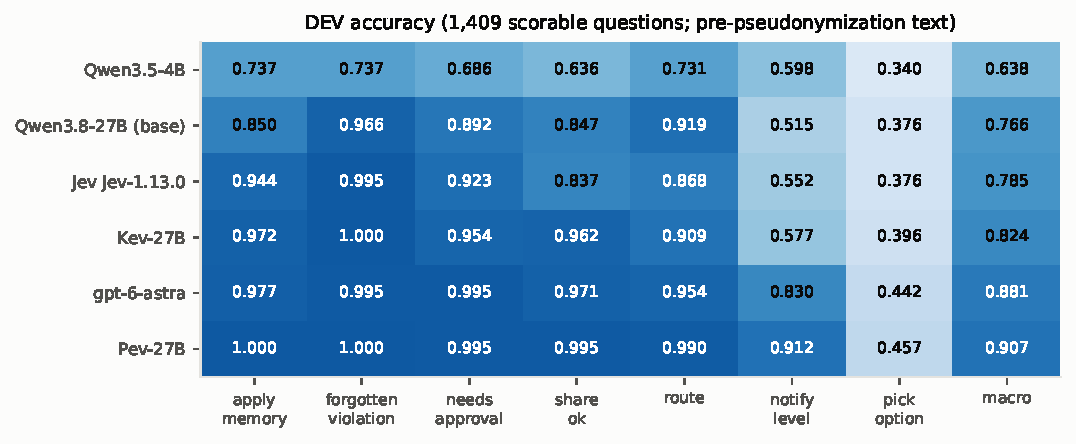
\includegraphics[width=0.9\linewidth]{figures/fig5_dev_references.pdf}
\caption{DEV accuracy per family and predictor.}
\label{fig:devref}
\end{figure}

\paragraph{Caveats.}
(1)~The local models are scored from label-token log-probabilities (Kev-27B from its own head) with a VAL-fitted
temperature; gpt-6-astra verbalises probabilities in a JSON answer and Jev returns them from its API. Accuracy
(argmax) is unaffected, but the Brier and ECE of the API models are uncalibrated, and they have no automation
threshold. (2)~The API models see each state once with all its questions; the local models see one question per
prompt. (3)~gpt-6-astra rendered DEV and so scores text it wrote itself. (4)~DEV was the hill-climb test set for the
adapter, so its DEV score carries selection bias (HIDDEN confirms it within 0.2~points). (5)~These numbers were computed
on the \textbf{pre-pseudonymization} DEV text; the released DEV is pseudonymized (person names, contact details and
user ids only; options and labels unchanged) and was not re-scored, so re-running on it may give slightly different
numbers. TEST (\sect\ref{sec:test}) is free of caveats (4) and (5), and its B half also of (3).

% ======================================================================================================================
\FloatBarrier
\section{Analysis and limitations}\label{sec:analysis}

\paragraph{\fml{pick_option} is unsolved and over-automated.}
The one family labelled by real behaviour (which item the user later rated $\geq 4$) moves from 0.398 to 0.431 on
HIDDEN (+3.3~points, CI [$-$3.1, +9.6]); on DEV every training landed between 0.38 and 0.46, and more data did not help.
Every model measured on DEV scores between 0.34 and 0.46 against a chance level of 0.28. Worse, the adapter's
VAL-fitted threshold accepts half of the HIDDEN \fml{pick_option} questions with a realized error of 44.7\% (43.8\% on
DEV), so the 5\% automation budget does not transfer to this family. A deployment must keep \fml{pick_option} as
\emph{ask the user}, whatever the confidence. The residual \fml{pick_option} shortcuts (DEV centroid +2.5, HIDDEN
medoid +3.3~points) are as large as the adapter's gain, so we claim no \fml{pick_option} progress. TEST confirms the
picture: all six models score 0.41--0.48 next to a ``priciest'' shortcut of 0.347 (chance 0.276), the adapter is not
significantly ahead of gpt-6-astra or B0, and its accepted \fml{pick_option} questions have a realized error of 37\%.
Predicting real choices probably needs richer user-history context rather than more training rows.

\paragraph{Rule-derived families saturate.}
Six families are deterministic functions of seeded rules and the KB; the adapter reaches 0.97--1.00 on them on both DEV
and HIDDEN. This shows that the rules can be learned from rendered text, including buried, overridden and
private-style variants, not that the model has general judgement about approvals or privacy; real users' rules will be
messier than our generators.

\paragraph{The guard gain is partly in-distribution.}
The general mix comes from \code{decision-v2/train}, the train side of the suite whose test side is the
\code{decision-v7} guard (disjoint items, n-gram audited). The +1.4-point guard result shows that the forgetting seen in
round~1 is stopped, not that general decision ability improved; MNLI and Banking77 still drop.

\paragraph{Renderer home advantage.}
gpt-6-astra rendered TRAIN, VAL, DEV and the public half of HIDDEN, and is also a reference: on DEV it scores text it
wrote, and the adapter was trained on that renderer's style. TEST addresses both sides. Its B half is rendered by a
different model, so the adapter is tested outside its training distribution and gpt-6-astra loses any familiarity
advantage; the A/B difference per model measures the effect directly. On TEST no home advantage is visible:
gpt-6-astra scores 0.876 on its own renders and 0.871 on Claude's ($-$0.4~points), the adapter 0.913 and 0.917 (+0.5),
and the adapter's lead over gpt-6-astra is +3.7~points on A and +4.6 on B. The renderer effect is also small for B0
(+0.7), Kev-27B ($-$0.4) and Jev (+1.7); only Qwen3.5-4B scores clearly higher on the B half (+4.9).

\paragraph{LLM-rendered text.}
Every state is LLM-rendered from structured facts under verbatim anchor constraints, and the memory facts are
LLM-extracted (with verbatim evidence). Real user text is noisier, longer-range and contradictory in ways our override
and buried variants only approximate. The synthetic rules attached to real histories are a modelling device, not data
about real people.

\paragraph{DEV numbers predate pseudonymization.}
All DEV numbers in this report (\sect\ref{sec:stats}, \sect\ref{sec:validity}, \sect\ref{sec:dev},
\sect\ref{sec:devref}) were scored on the DEV text \textbf{before} pseudonymization. The released DEV differs only in
person names (mostly inside Enron distractor text), contact details and user ids, and was not re-scored. The adapter
was likewise trained on pre-pseudonymization TRAIN rows (SFT rows SHA-256 \code{046a2ddb...}).

\paragraph{Released TEST equals scored TEST.}
TEST was pseudonymized before any model was scored: the scored file (\code{test.jsonl}, SHA-256 \code{131d0927...79a3},
as recorded in \code{docs/TEST_RESULTS.json}) is the byte concatenation of the two released half files
(\code{test-a.release.jsonl} \code{b2fade97...}, \code{test-b.release.jsonl} \code{d7907b2a...}), so the released TEST
is the file every model was scored on.

\paragraph{Other limitations.}
One base model and one LoRA configuration; one seed for the final candidate (build variance measured at 0.3~points in
round~1); the hill-climb stopped after two rounds rather than three (\sect\ref{sec:deviations}); HIDDEN is reported only
in aggregate and not per style half; the API references are uncalibrated.

% ======================================================================================================================
\FloatBarrier
\section{Release}\label{sec:release}

\begin{table}[htb]
\caption{Released artifacts.}
\label{tab:release}
\centering\footnotesize
\begin{tabularx}{\linewidth}{@{}>{\raggedright\arraybackslash}p{2.4cm} L >{\raggedright\arraybackslash}p{4.4cm}@{}}
\toprule
Artifact & Content & Access and license \\
\midrule
Code & \code{packages/personal-decisions} (KB builder, splits, families, renderer, anchor verifier, privacy scan,
  \code{export-release}), \code{packages/decision-eval} (scorers, calibration, gates, statistics), \code{training/}
  (standalone trainer and adapter evaluation), \code{scripts/} (data acquisition, general mix) & Apache-2.0 \\
Data & Pev-Bench: TRAIN (our records only; the Kev general-mix rows are not redistributed, only their ids
  and hashes), VAL, DEV and TEST (A and B halves), pseudonymized, on Hugging Face & Gated, research-only; CC-BY-NC-4.0
  for our contributions (labels, synthetic rules, structure, rendered wording); third-party text remains under its
  owners' terms; OpenFlights data under ODbL 1.0 / DbCL 1.0 (notice included) \\
Pseudonymization key & \code{release/pseudonym_key.txt}, which makes \code{export-release} exactly reproducible &
  Published; the pseudonymization is reversible by design, and all sources are already public \\
Weights & Pev-27B: the r2-mix LoRA adapter on \code{Qwen/Qwen3.8-27B} (SHA-256 \code{6b07a7d3...}) & Gated,
  non-commercial research licence \\
Report & This document, its tables and figures & CC-BY-4.0 \\
\bottomrule
\end{tabularx}
\end{table}

Table~\ref{tab:release} lists the released artifacts. \textbf{HIDDEN is not released.} The HIDDEN result in
\sect\ref{sec:hidden} comes from the single one-shot run, which produced aggregate-only outputs; the sealed set was
deleted after the run. Questions and removal requests: \texttt{research@envloop.ai}. Source citations: Amazon Reviews
2023~\citep{hou2024amazon}; UCTopic~\citep{li2022uctopic} and Personalized Showcases~\citep{yan2023showcases} for
Google Local; OpenFlights~\citep{openflights}; the CMU Enron email corpus~\citep{klimt2004enron}; Kev~\citep{kev}.

% ======================================================================================================================
\FloatBarrier
\bibliographystyle{plainnat}
\bibliography{refs}

% ======================================================================================================================
\clearpage
\appendix

\section{Hyperparameters}\label{app:hparams}

\begin{table}[h]
\caption{Training and scoring settings of the released adapter.}
\label{tab:hparams}
\centering\footnotesize
\begin{tabularx}{\linewidth}{@{}>{\raggedright\arraybackslash}p{4.2cm} L@{}}
\toprule
Setting & Value \\
\midrule
Base model & \code{Qwen/Qwen3.8-27B} @ \code{1d4bf0f2ff6012fd82039f2fa52739d0dd7c60c0}, bf16, no quantisation \\
Method & LoRA SFT, loss on the single option-label token \\
LoRA & $r$ 16, $\alpha$ 32, dropout 0.05; targets \code{self_attn.{q,k,v,o}_proj},
  \texttt{linear\_attn.\{in\_proj\_qkv,\allowbreak in\_proj\_z,\allowbreak in\_proj\_a,\allowbreak
  in\_proj\_b,\allowbreak out\_proj\}}, \code{mlp.{gate,up,down}_proj} in every layer \\
Optimiser & AdamW, learning rate $5 \times 10^{-5}$, 24 warm-up steps, cosine decay \\
Batch & 1 per device $\times$ 8 gradient-accumulation steps \\
Steps & 776 (6,201 rows, one pass); checkpoint every 250 steps \\
Maximum length & 12,288 tokens (longest row 8,649; 8.44M prompt tokens in total) \\
Seed & 20260930 \\
Template & \code{direct} (VAL macro 0.759; \code{assistant} 0.748, \code{evidence} 0.742) \\
Temperature (VAL, NLL) & B0 1.675, adapter 2.772 \\
Automation threshold (VAL, 5\% budget) & B0 0.754, adapter 0.369 \\
Adapter archive & SHA-256 \code{6b07a7d36eba59b9cfd9cf440bdc5783}\allowbreak\code{f4fc12d4d726cfa5beef2462860d8d81}, 436\,MB \\
\bottomrule
\end{tabularx}
\end{table}

\section{Prompt template}\label{app:prompt}

The frozen \code{direct} template (\path{packages/decision-eval/decision_eval/templates/direct.txt}), filled per
question and wrapped as one user turn by the Qwen chat template with \code{enable_thinking=False}:

\begin{verbatim}
{state}

Question: {instructions}
{options}

Answer with {answer} only.
\end{verbatim}

\code{{options}} lists \code{A. <option>} lines for \code{choice}, \code{yes: <criterion>} and \code{no: <criterion>}
for \code{noul}, and \code{0: <level>}, \code{1: <level>}, \ldots{} for \code{score}. \code{{answer}} is ``yes or no''
or ``the label of exactly one option (A, B, C)'' (or ``\ldots{} level (0, 1, 2, 3)''). The model's next-token
log-probabilities over these single-token labels are the prediction.

\section{Per-family definitions}\label{app:families}

\begin{itemize}[leftmargin=1.2em]
\item \textbf{\fml{pick_option}} (choice, 3--5 options). Target: an item from a real later interaction rated
  $\geq 4$. Candidates: the target; the user's real later item of the same category rated $\leq 2$, when the target
  can still be balanced around it; and untouched items of the same category (restaurants: same city and Google
  category; products: the same subcategory when possible), drawn so that price, popularity, medoid and centroid
  distance do not single out the target. Override: an older budget is lifted by a newer one that covers every
  candidate. Removed: soft label.
\item \textbf{\fml{needs_approval}} (noul). Spend threshold in force at the time, new-recipient rule,
  irreversible-action rule. Override: a threshold change flips the answer. Removed: soft 0.5.
\item \textbf{\fml{apply_memory}} (noul). Whether the memory fact's category matches the request; negatives are other
  product departments or unrelated tasks (never another restaurant category).
\item \textbf{\fml{forgotten_violation}} (noul). Whether the action relies on a fact the user asked to forget. Removed:
  the forget request is withheld and the label is false.
\item \textbf{\fml{share_ok}} (noul). Recipient clearance $\geq$ the fact's privacy level. Override: the fact is
  re-marked. Removed: soft 0.5.
\item \textbf{\fml{notify_level}} (score, 4 levels). Event urgency capped by the event type's maximum, quiet hours and
  the meeting cap at the event's arrival time, with VIP bypass. Override: quiet hours change. Removed: the urgency is
  withheld and the soft label is uniform over the reachable levels, so the question is never scored.
\item \textbf{\fml{route}} (choice, 6 options). The needed service if it is connected, else \code{ask_user} (also for
  OpenFlights city names ambiguous across countries); label names are scheduled in equal sixths. Override: dated
  connections and disconnections.
\end{itemize}

\section{Costs}\label{app:costs}

\begin{table}[h]
\caption{GPU and API usage of the whole project, including failed and abandoned attempts.}
\label{tab:costs}
\centering\footnotesize
\begin{tabularx}{\linewidth}{@{}L >{\raggedright\arraybackslash}p{4.3cm} >{\raggedleft\arraybackslash}p{1.7cm}@{}}
\toprule
Item & Resource & Cost (USD) \\
\midrule
Baseline evaluation (B0, Qwen3.5-4B and Kev-27B on VAL, DEV and the guard) & H100 spot, 08:02--09:03 UTC & 2.00 \\
Round 1, seed A & H100, 2.33\,h & about 9 \\
Round 1, seed B & H100, 2.45\,h & about 13 \\
Round 2, mix (final adapter) & H100, 2.76\,h & about 11 \\
Round 2, 7k & H100 spot, 2.98\,h & about 10.9 \\
HIDDEN gate & H100, 37\,min & about 2.5 \\
Failed or abandoned attempts: two evicted or aborted 7k runs ($\approx$6.7 + $\approx$8), an aborted seed-B run
  ($\approx$7), a step-limit failure ($\approx$1.6), an early SSH failure ($\approx$0.1) & --- & about 23.4 \\
Infrastructure staging & --- & about 2 \\
GPU subtotal through the HIDDEN gate (sum of the rows above) & & about 73.8 \\
TEST reproduction check (B0, adapter, Qwen3.5-4B and Kev-27B on DEV) & A100 80GB, 14:12--15:08 UTC & about 1.15 \\
TEST evaluation of the four local models & H100 80GB, 15:14--16:22 UTC & about 3.80 \\
\textbf{GPU total for the project} (73.8 + 1.15 + 3.80) & & \textbf{about 78.8} \\
\midrule
Jev on DEV & 630 requests, 1.42M input tokens & 0.06 \\
Jev on TEST & 980 requests, 2.33M input tokens & 0.10 \\
gpt-6-astra on TEST (reference) & 980 records (982 calls), 1.91M input and 0.12M output tokens & not priced \\
gpt-6-astra for TEST construction & memory extraction 829 requests (0.52M input, 0.24M output); A-half rendering 490
  requests (0.54M input, 0.33M output) & not priced \\
gpt-6-astra on DEV (reference) & 630 requests, 1.16M input and 0.08M output tokens & not priced \\
gpt-6-astra memory extraction (KB) & 3,426 requests, 2.14M input and 0.96M output tokens & not priced \\
gpt-6-astra rendering, TRAIN and VAL (all runs) & 5.82M tokens & not priced \\
gpt-6-astra rendering, DEV (all runs) & 2.29M tokens & not priced \\
\bottomrule
\end{tabularx}
\end{table}

Per-row GPU figures (Table~\ref{tab:costs}) are estimates from hourly price $\times$ runtime (provider invoices are
authoritative); an earlier running total in the authors' run records overstated the sum by an arithmetic error
(\code{docs/RESULTS.md}, Errata). The project budget was capped at \$2,000 for GPU and API usage together.

\section{Compute}\label{app:computedetail}

Every training and evaluation job ran on one NVIDIA H100 80GB GPU; the managed training jobs used checkpoint resume.
Scoring loads the bf16 weights (about 52\,GB) with the rank-16 adapter unmerged. One predictor over DEV scores 1,626
prompts, 3.0M prompt tokens under the \code{direct} template (median 954, 95th percentile 6,184, maximum 8,145 tokens
per prompt). Software: torch 2.14.0~\citep{paszke2019pytorch}, transformers 5.17.0~\citep{wolf2020transformers}, peft
0.21.1~\citep{peft} (\code{docs/VERSIONS.md}).

\section{TEST run}\label{app:testrun}

\paragraph{Reproduction check.}
Before TEST, the four local models were re-run on DEV on an A100 with the same scorer, template, adapter and
temperatures. Argmax agreement with the frozen DEV predictions was 1,616/1,626 for B0 (macro 0.768 against 0.766) and
1,619/1,626 for the adapter (0.909 against 0.907; Brier and coverage identical to three decimals). Every flip was a
near-tie in the frozen predictions (top-2 gap $\leq 0.054$); the cause is bf16 kernels on a different GPU. All local
TEST predictions were therefore produced on one machine, so the TEST comparison is internally consistent. The scoring
command reproduces the DEV reference comparison of \sect\ref{sec:devref} exactly.

\paragraph{Incident.}
During the local TEST run on one H100, an SSH drop ended the local driver of the B0 run while B0 kept running on the
GPU machine to completion (one run). The driver loop then started the adapter on the still-busy GPU; it failed with a
CUDA out-of-memory error while loading weights, before any question was scored, produced no output and was discarded.
The remaining models ran from a detached queue on the GPU machine, each once. Every model therefore produced exactly
one prediction set, and all six sets were hashed and frozen (\code{docs/TEST_PREDICTIONS.sha256}, 2026-10-01 16:22
UTC) before any scoring. gpt-6-astra needed two extra calls within its 980 record requests (parser retries, as on
DEV); neither API model had an unscorable record. Per-model runtimes on the H100: B0 1,039\,s, adapter 1,050\,s,
Kev-27B 846\,s, Qwen3.5-4B 221\,s.

\end{document}
